\section{What We Discovered}

\begin{figure*}
  \centering
  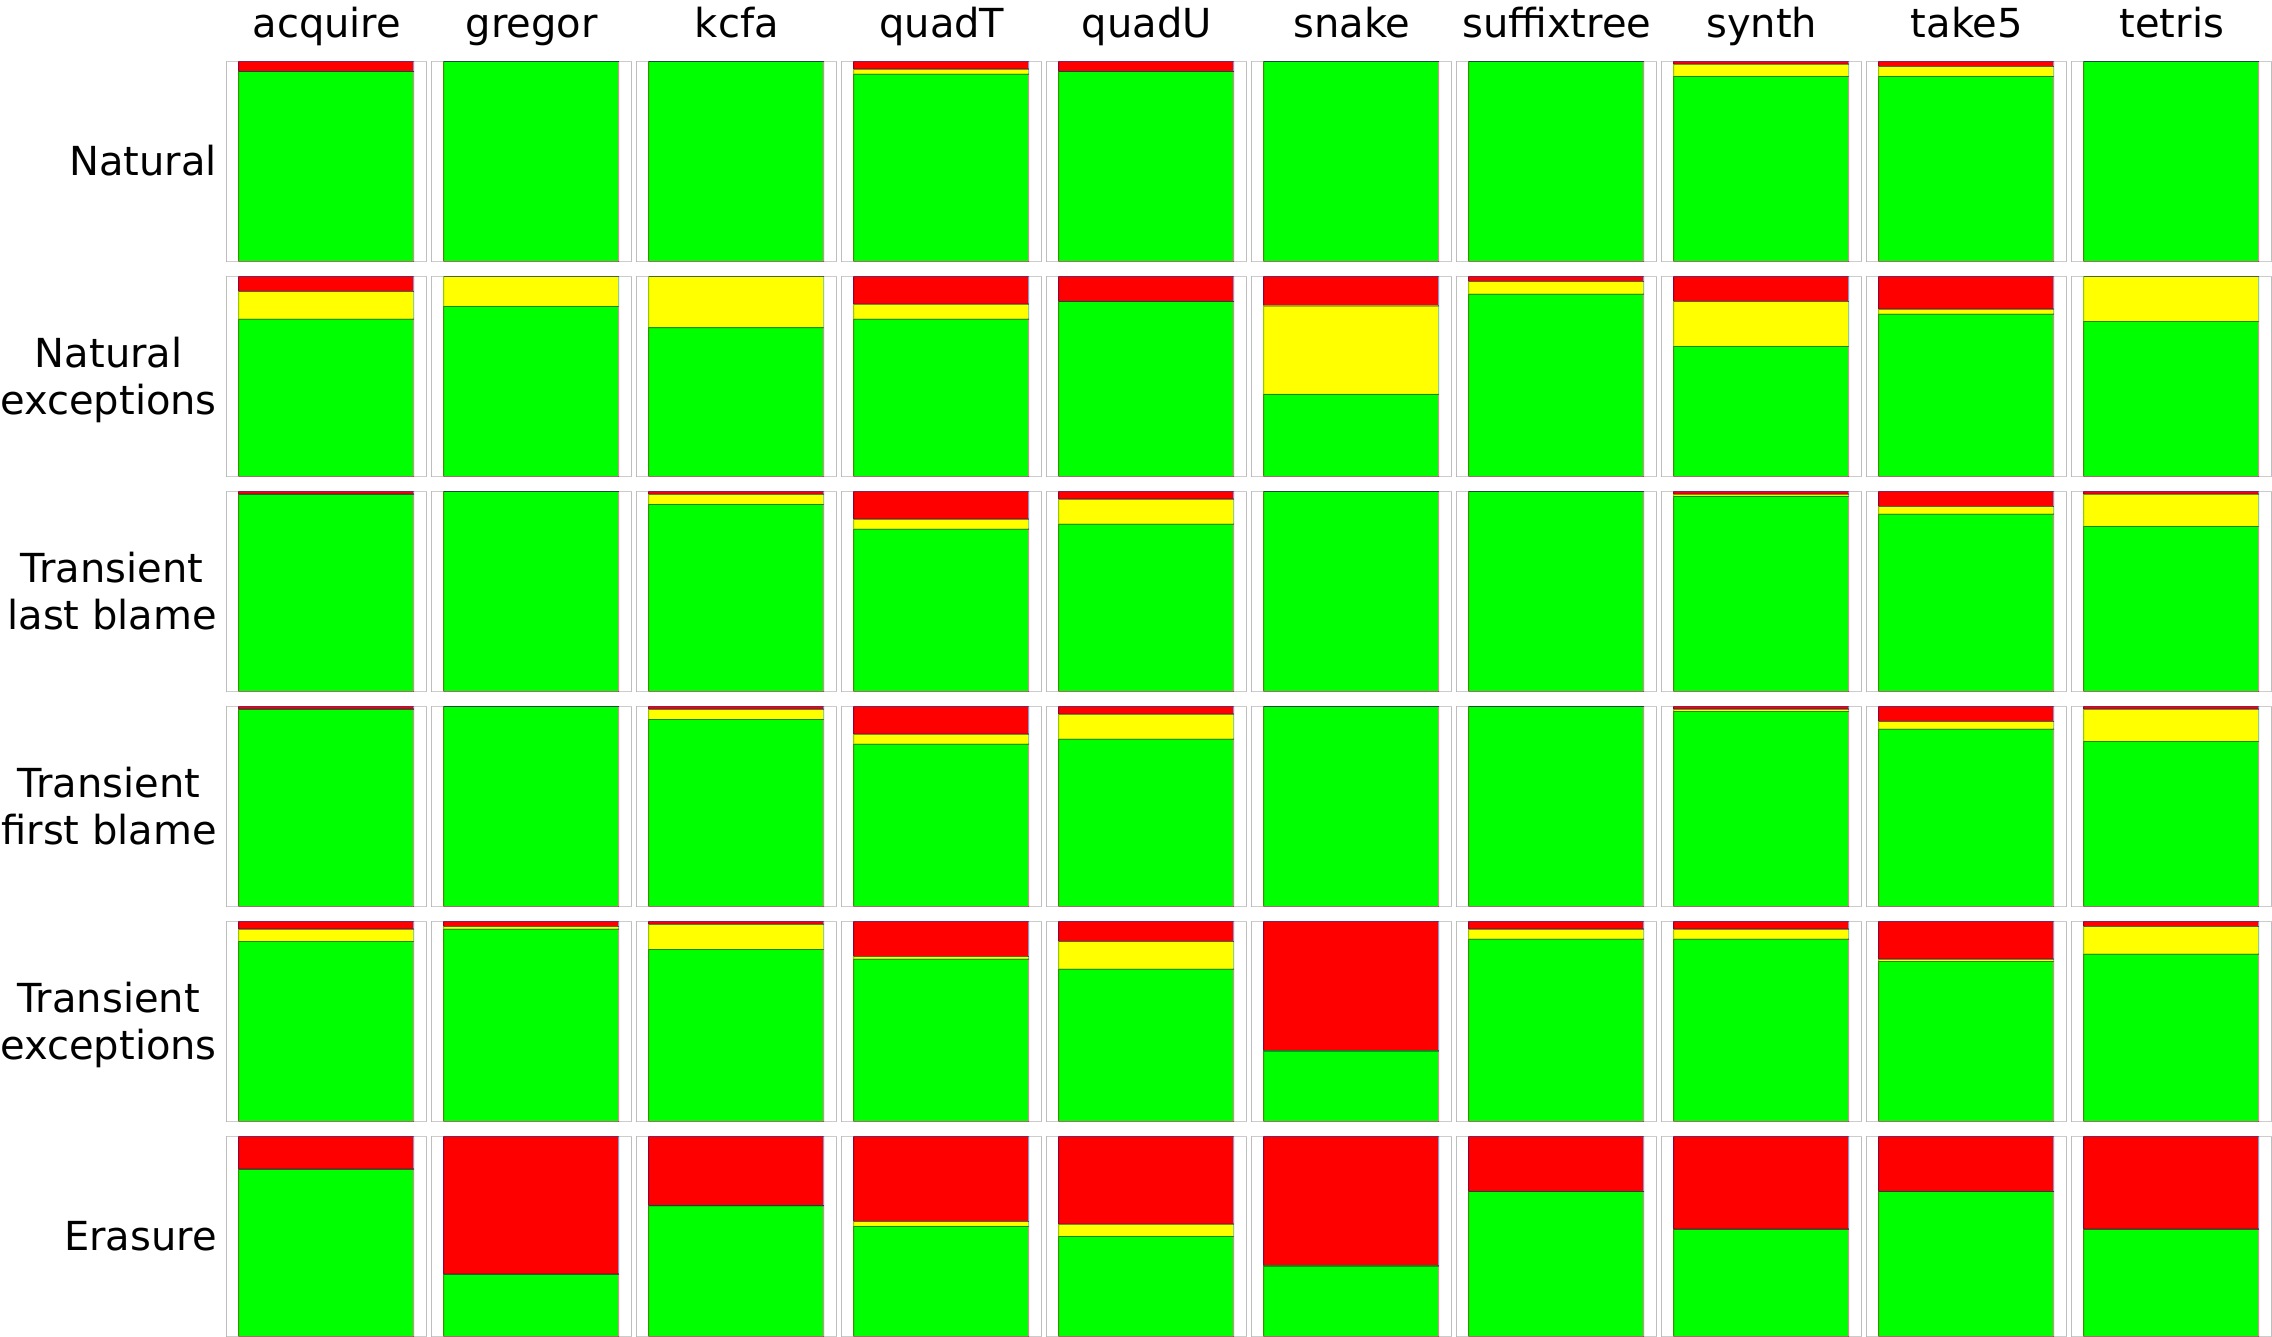
\includegraphics[width=0.7\textwidth]{./plots/usefulness-table}
  \caption{Usefulness: Each cell depicts the proportion of a benchmark's mutants for which a mode is always useful (green), sometimes useful (yellow), and never useful (red).}
  \label{fig:usefulness-table}
\end{figure*}

\begin{figure*}
  \centering
  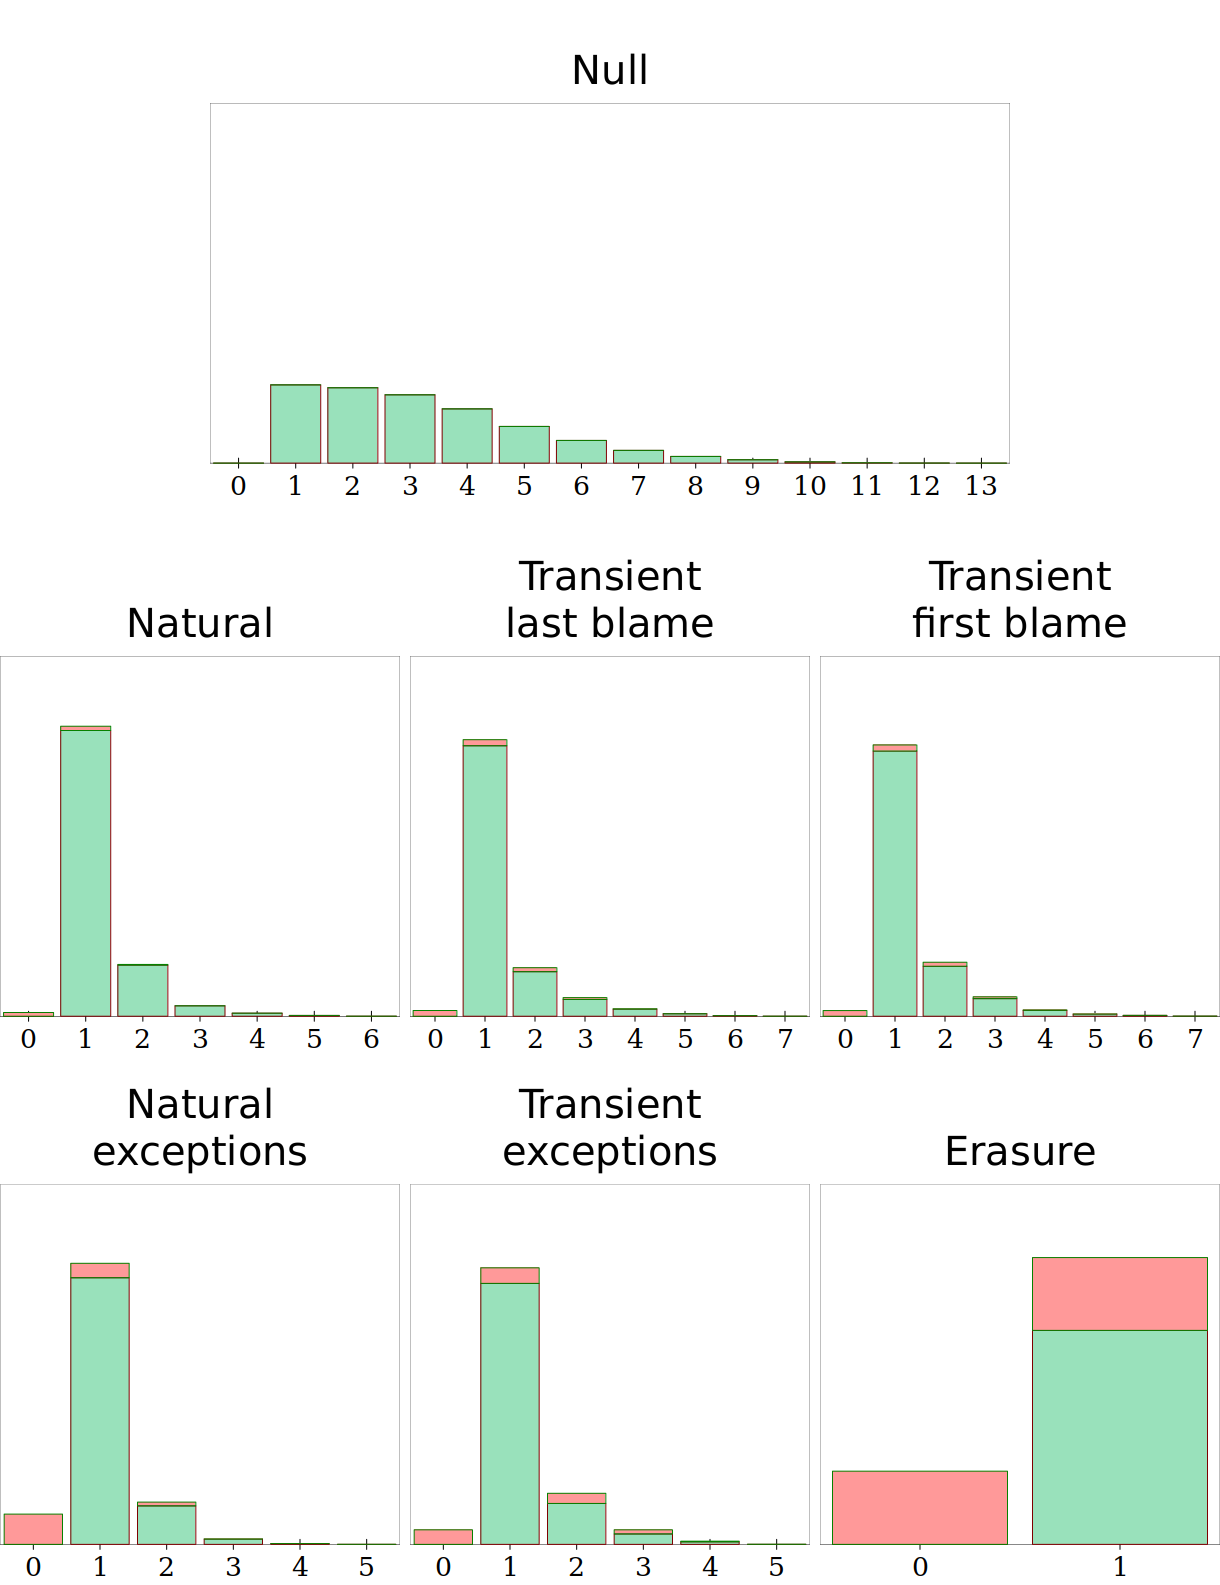
\includegraphics[width=0.95\textwidth]{./plots/bt-lengths-table}
  \caption{Programmer effort: Each cell depicts the distribution of trail
  lengths for a given mode and a benchmark's mutants starting from trails
  of length 0.}
  \label{fig:effort-table}
\end{figure*}

\begin{figure}
  \centering
  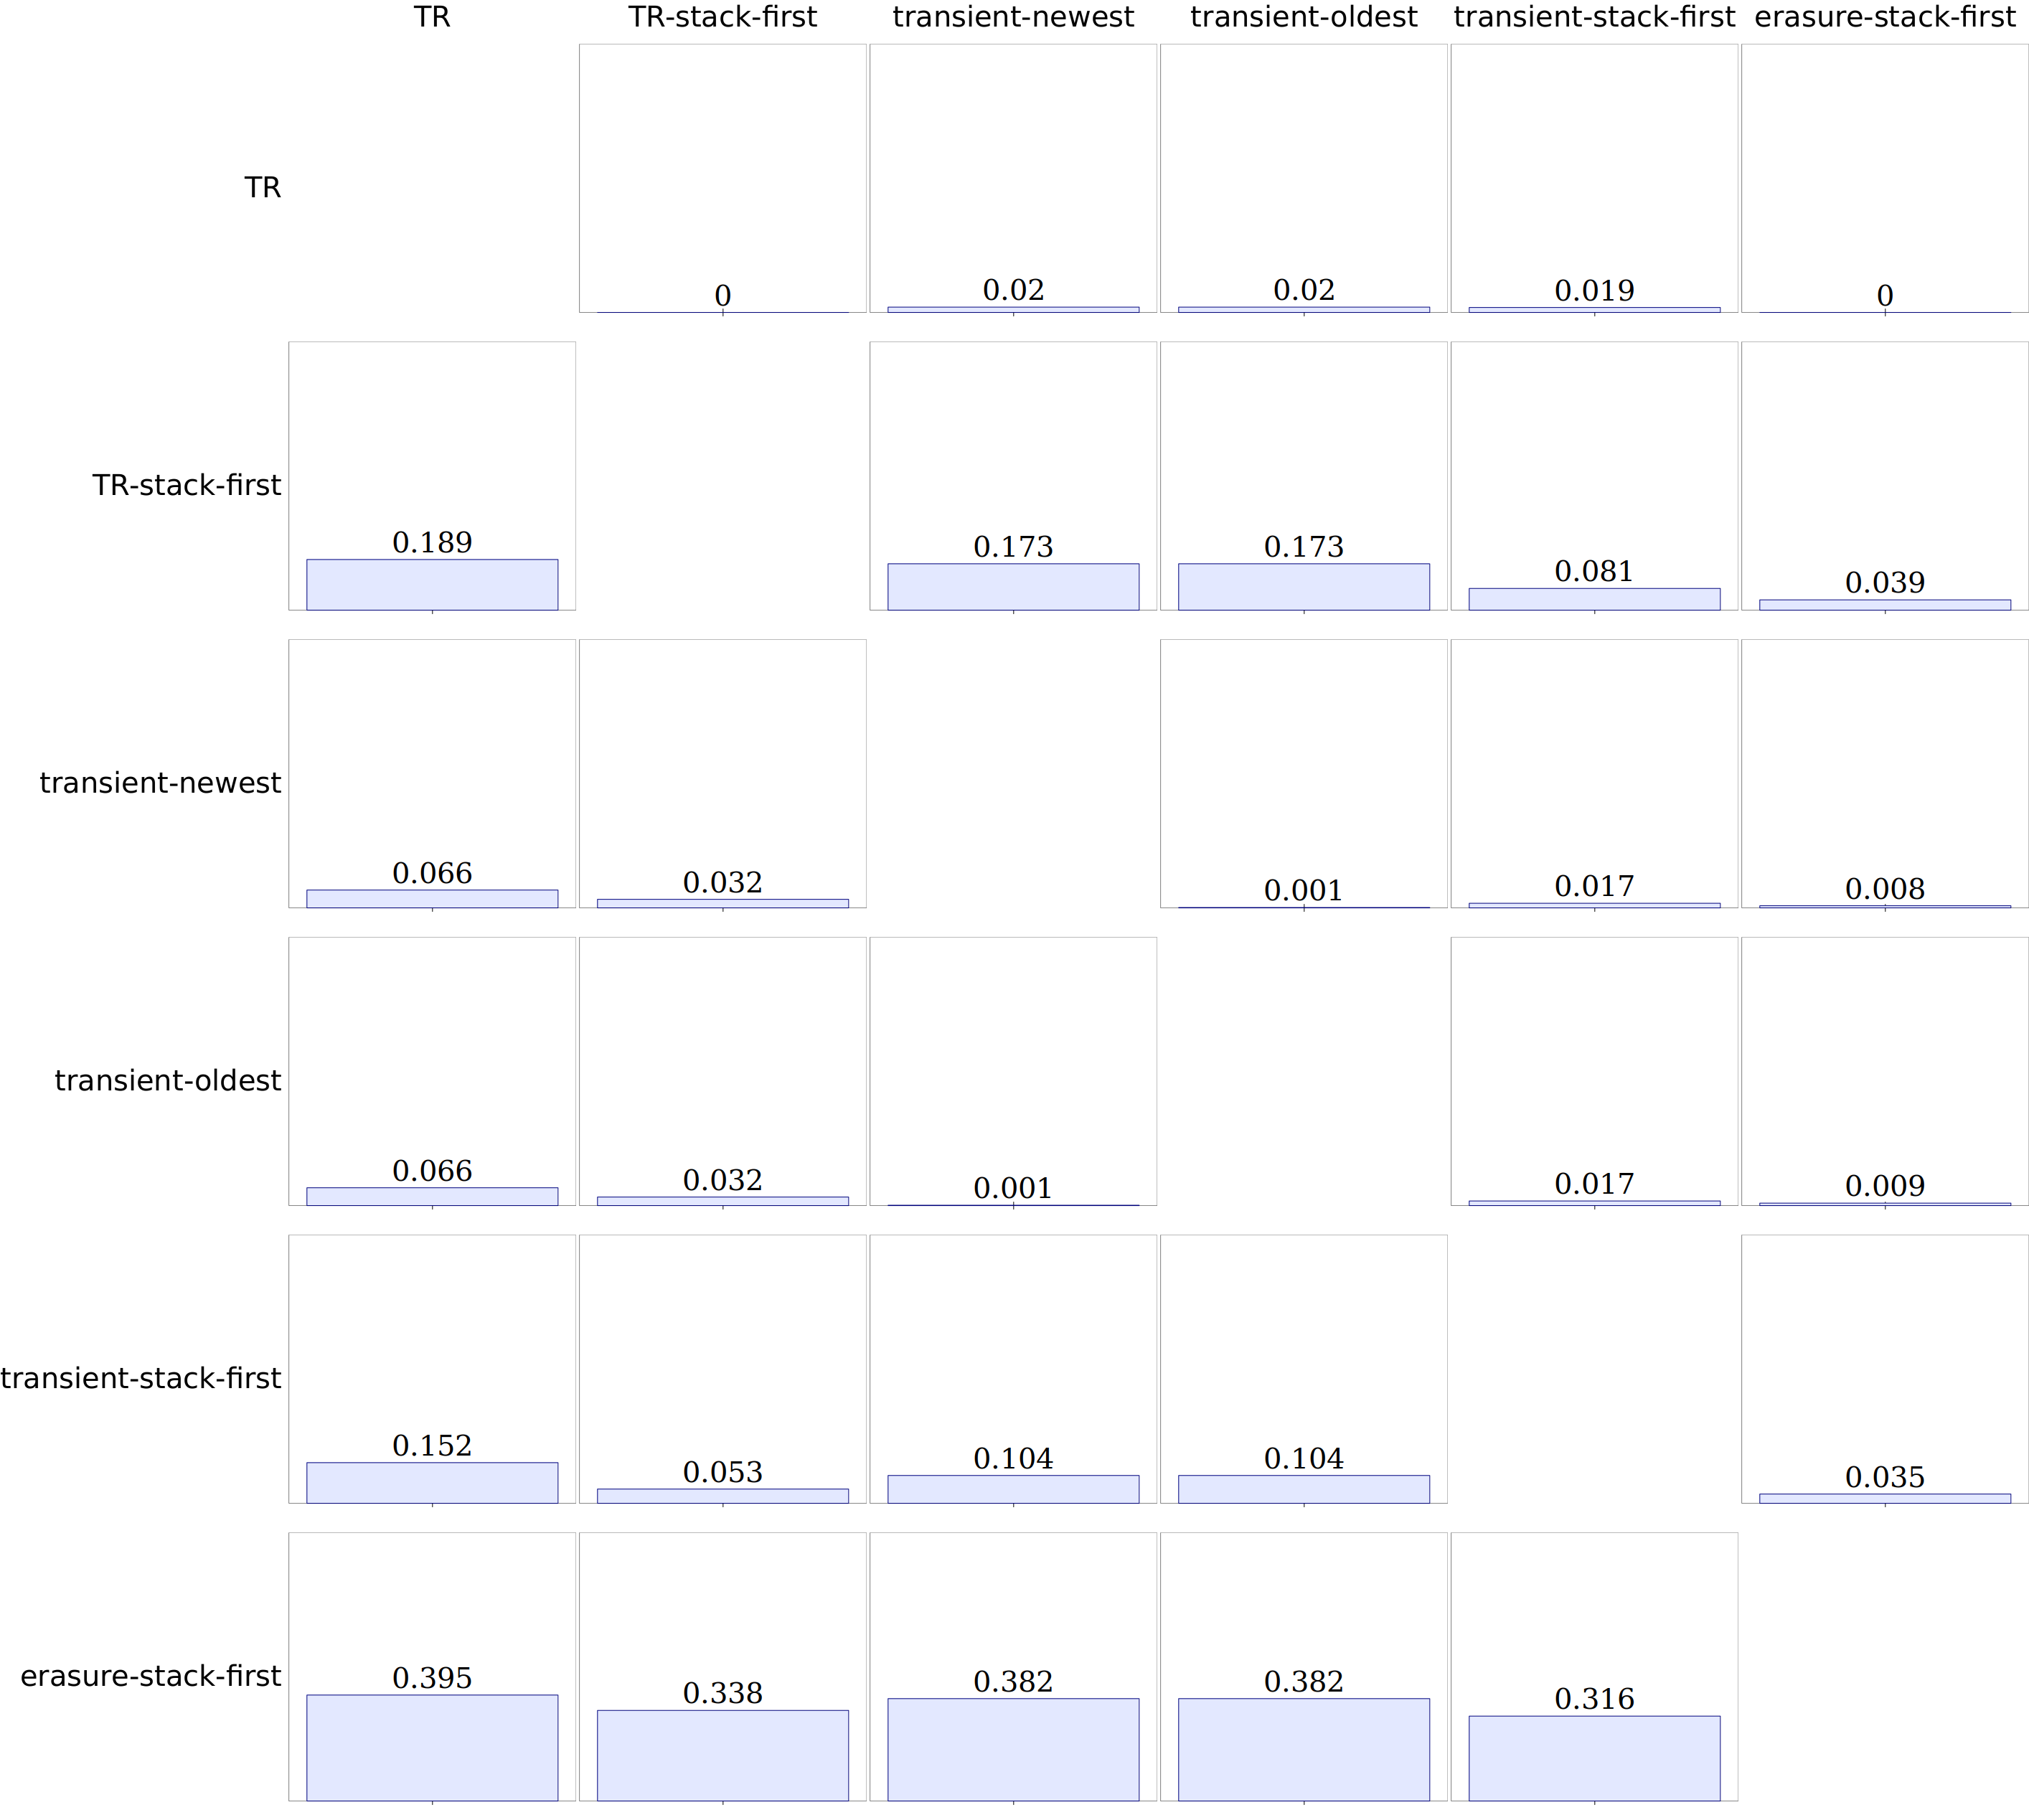
\includegraphics[width=0.45\textwidth]{./plots/avo-matrix}
  \caption{Usefulness comparisons: Each cell depicts the percentage of a
  benchmark's mutants for which the row mode is more useful than the column mode.}
  \label{fig:avo-matrix}
\end{figure}

We present our results according to the three dimensions for assessing the utility of blame described in section~\ref{sec:rational}: how often blame is always, sometimes, and never useful (figure~\ref{fig:usefulness-table}); programmer effort (figure~\ref{fig:effort-table}); and how often one mode adds value over another mode (figure~\ref{fig:avo-matrix}).
In this section we analyze each of these dimensions in turn, and in the next we discuss the analysis's high level conclusions.

Figure~\ref{fig:usefulness-table} breaks down how often blame is useful (as defined in section~\ref{sec:rational}) for every benchmark and every mode of the rational programmer.
Each mode corresponds to a row of the table, while the columns correspond to our benchmarks.
Each cell plots the proportion of a benchmark's mutants for which a mode is always useful (green), sometimes useful (yellow), and never useful (red).
Comparing the overall pattern of one row to the others provides a broad understanding of how the usefulness of that mode compares with the others.
For instance, the large proportions of red across Erasure indicates that for many mutants it is never useful.

Figure~\ref{fig:effort-table} shows the distribution of trail lengths for every benchmark and every mode of the rational programmer.
The modes correspond to rows and columns to benchmarks, like figure~\ref{fig:usefulness-table}.
In this case, however, the cells plot trail length distributions starting from length zero in the leftmost bar and going up by one for each bar to the right.
Each bar is broken into two sub-bars, which are color-coded to indicate the proportion of trails within that bar which are successful (green) and not (red).
Again, comparing the rows of the table provides a high level view of how the lengths of trails for each mode tend to differ.
For example, the stark difference between the Null mode's distribution and that of every mode illustrates how using blame information (as opposed to randomly selecting components to type) dramatically shortens the rational programmer's search.
The Null distributions look approximately normal \emdash reflecting that the Null mode always selects a random next component to type \emdash but shifted left, reflecting that our scenarios start with a randomly-selected subset of components already typed.
On the other hand, all of the other modes have distributions that are significantly more concentrated around trails of length one and two.

Finally, figure~\ref{fig:avo-matrix} shows a head-to-head comparison of each mode against every other mode.
Each cell of the table compares one mode to another using section~\ref{sec:rational}'s definition of a mode \emph{adding value over} another mode.
In particular, a cell in row $R$ and column $C$ plots the percentage of mutants for which $R$ adds value over $C$.
For example, the second cell in the row of Natural shows that Natural adds value over Natural exceptions for 18.9\% of all the mutants we consider.
Reading across a given row $R$ provides an overview of how $R$ compares to every other mode;
the higher the bars, the more mutants for which $R$ is strictly more useful than the other modes.
Reading down a given row $C$ provides an overview of how every other mode compares to $C$;
the higher the bars, the more mutants for which $C$ is strictly less useful than the other modes.

